\documentclass[twoside,letterpaper]{refart}

% \usepackage{fullpage}
\usepackage{graphicx}
\usepackage{verbatim}
\usepackage{natbib}
\usepackage{outlines}
\usepackage{enumitem}
\usepackage{lineno}
\usepackage{subfigure}
\usepackage{booktabs}
\usepackage{wrapfig}
\usepackage{ulem}
\usepackage[hidelinks]{hyperref}
\usepackage{todonotes}
\usepackage{floatrow}
\usepackage[export]{adjustbox}
\usepackage{caption}
\usepackage{color}
\usepackage{placeins}
\usepackage{changepage}

%\usepackage{stfloats}
%\usepackage[labelformat=empty]{subfig}
%\usepackage{wasysym}

    % See p.105 of "TeX Unbound" for suggested values.
    % See pp. 199-200 of Lamport's "LaTeX" book for details.
    %   General parameters, for ALL pages:
    \renewcommand{\topfraction}{1}	% max fraction of floats at top
    \renewcommand{\bottomfraction}{1}	% max fraction of floats at bottom
    %   Parameters for TEXT pages (not float pages):
    \setcounter{topnumber}{2}
    \setcounter{bottomnumber}{2}
    \setcounter{totalnumber}{6}     % 2 may work better
    \setcounter{dbltopnumber}{2}    % for 2-column pages
    \renewcommand{\dbltopfraction}{0.9}	% fit big float above 2-col. text
    \renewcommand{\textfraction}{0.07}	% allow minimal text w. figs
    %   Parameters for FLOAT pages (not text pages):
    \renewcommand{\floatpagefraction}{0.7}	% require fuller float pages
    % N.B.: floatpagefraction MUST be less than topfraction !!
    \renewcommand{\dblfloatpagefraction}{0.7}	% require fuller float pages

\usepackage{makeidx}
\usepackage{ifthen}
\def\bs{\char'134 } % backslash in \tt font.
\newcommand{\ie}{i.\,e.,}
\newcommand{\eg}{e.\,g..}
\DeclareRobustCommand\cs[1]{\texttt{\char`\\#1}}

\pagestyle{myfootings}
\markboth{SuperCO$_2$ System Manual}%
		{SuperCO$_2$ System Manual}

\makeindex

\setcounter{tocdepth}{2}


%\usepackage{endfloat}

\setenumerate[1]{label=\Roman*.}
\setenumerate[2]{label=\Alph*.}
\setenumerate[3]{label=\roman*.}
\setenumerate[4]{label=\alph*.}

%\linenumbers


\newcommand{\dioxide}{$\mathrm{CO}_2$\ }
\newcommand{\water}{$\mathrm{H}_2\mathrm{O}$\ }
\newcommand{\super}{Super$\mathrm{CO}_2$\ }
\newcommand{\supertitle}{SuperCO$_\mathrm{\textbf{2}}$\ }



\begin{document}



\begin{titlepage}
	\thispagestyle{empty}
		\begin{nolinenumbers}
			\noindent
			
			\begingroup
				\vspace*{\fill}
				\begin{center}
				\vspace{5mm}
				\hspace{-50mm}
				{\Huge \textsf{\textbf{\supertitle System Manual}}}
				\vspace{2mm}
				\hbox{
					\hspace{-55mm}
					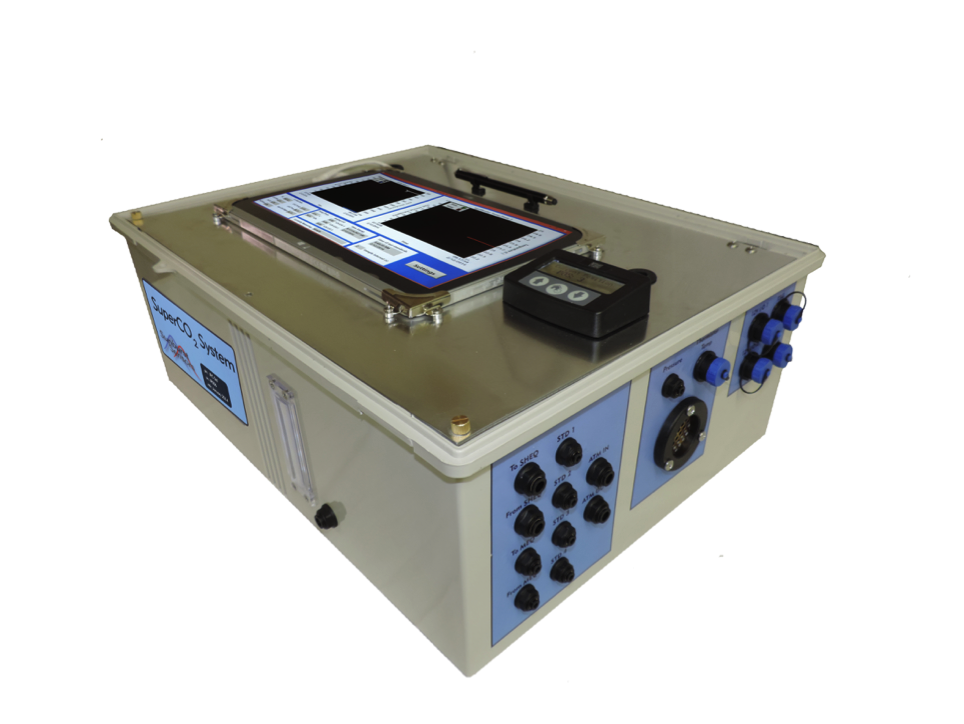
\includegraphics[scale=1.1]{Title.png}
				}
				\end{center}
				\vspace*{\fill}
			\endgroup

			\begin{minipage}[b]{0.5\hsize}
			\raggedright
			\hspace{-50mm}
			
\includegraphics[scale=0.6]{SBlogo.jpg}
			\end{minipage}
			\noindent
			\begin{minipage}[b]{0.5\hsize}
			\raggedleft
			\small
			Sunburst Sensors, LLC\\
			1226 W Broadway Ave\\
			Missoula, MT 59802\\
			+1 406 532 3247\\
			\end{minipage}
			
		\end{nolinenumbers}
\end{titlepage}

\newpage\null\thispagestyle{empty}\newpage

\newpage

\addtocontents{toc}{\protect\thispagestyle{empty}}

\tableofcontents

\clearpage

\newpage\null\thispagestyle{empty}\newpage

\setcounter{page}{1}


\section{\supertitle System Description}

The \super System is a high frequency p\dioxide measurement system for use shipboard or in the laboratory. It operates on the principle of equilibrating a gas stream to match the partial pressure of the dissolved \dioxide in a liquid stream, measuring the gas in parts per million (ppm) using a Licor\,840A.  The \super system allows periodic atmospheric readings and checks of the Licor\,840A using gas standards (not provided by Sunburst Sensors, LLC).


\subsection{Principle of Operation}

The \super System operates by equilibrating the \dioxide in a low volume gas stream with the \dioxide dissolved in a higher volume water stream using either a showerhead type equilibrator or a contactor type equilibrator.  The showerhead is more preferable in murky, dirty water that would be found in an estuary or other productive area, whereas the contactor offers greater simplicity and works very well in clean water.  The contactor can be used in water that is less clean by utilizing a filter.

	\begin{figure}[h]
	\hbox{
		\hspace{-54mm}
		\floatbox[{\capbeside\thisfloatsetup{capbesideposition={left,top},capbesidewidth=4cm}}]{figure}[\FBwidth]
		{\caption{Left side of the \super system (cooling fan, power connection, power switch, and USB connection).}\label{fig:Fig1}}
		{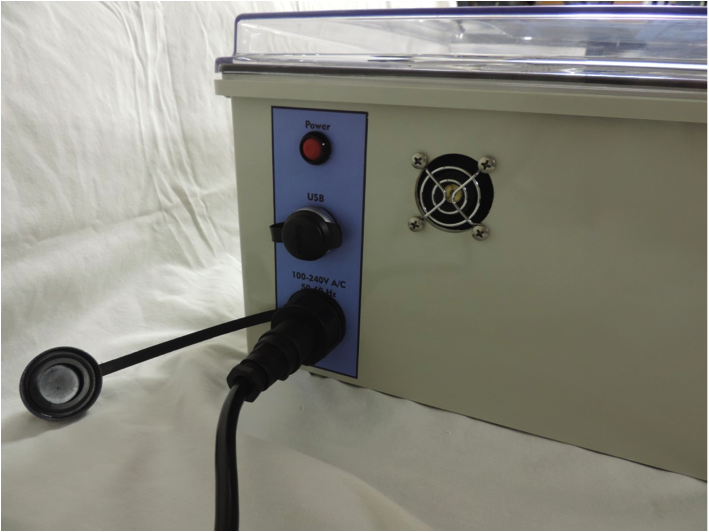
\includegraphics[width=\textwidth, left]{Fig1.png}}
	}
	\end{figure}


\subsection{Showerhead Equilibrator}

In the showerhead equilibrator (SHEQ) $\sim$\,1000\,mL/min of air is recirculated through the equilibrator while water is sprinkled through the air so that the air equilibrates with the water.  A small volume of air is diverted from the loop to the Licor\,840A for measurement and is replaced by make-up air from a low \dioxide source.  Care should be taken to have the make-up air inlet away from likely \dioxide sources � including respiration or exhaust gases.  Allowing these gasses into the inlet will drive the \dioxide high and the system will require time to re-equilibrate.  It is best to have make-up air come from outside or from a room with relatively low ($<$\,400\,ppm) \dioxide levels. It is recommended that the make-up air be teed off of the exhaust line of the atmospheric air.


\subsection{Membrane Equilibrator}

The membrane equilibrator (MEQ) uses a Liqui-Cel membrane contactor (2.5\,x\,8, G453) to exchange gas across a lumen.  Water flows on the outside of the lumen while gas flows in the opposite direction on the inside of the lumen.  While these products are typically used to add/remove dissolved gases, their principle of operation allows equilibration of a gas stream to the liquid stream�s p\dioxide level. This can be achieved if the flow ratio (liquid/gas) is large and the concentration gradient is not too large ($<$\,1000\,ppm). In the \super system, a seawater flow rate of $\sim$\,4\,L/min with a sample gas rate of $\sim$\,50\,mL/min assures that equilibration will occur at gradients up to 1000\,ppm, which covers most circumstances.  If gradients greater than 1000\,ppm are expected the liquid flow rate should be increased.

	\begin{figure}[h]
		\hbox{
			\hspace{-54mm}
			\floatbox[{\capbeside\thisfloatsetup{capbesideposition={left,top},capbesidewidth=4cm}}]{figure}[\FBwidth]
			{\caption{Front view of the \super system showing flow meter and exhaust port.}\label{fig:Fig2}}
			{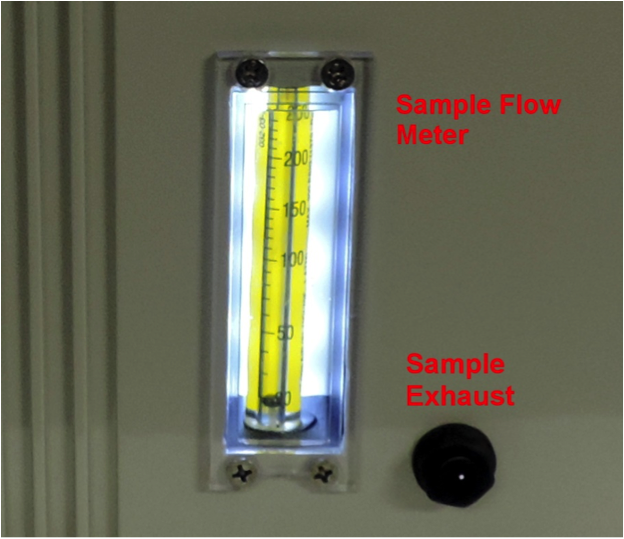
\includegraphics[width=\textwidth, left]{Fig2.png}}
		}
	\end{figure}


\section{Overview of \supertitle System}


\subsection{Power}

The \super system can use either 115--120\,VAC @ 60\,Hz or 220--240\,VAC @ 50\,Hz.  For 220--240\,VAC @ 50\,Hz operation the internal power supply must be switched accordingly. A power cord with a Bulgin connector is supplied and plugs into the left hand side of the system (Figure \ref{fig:Fig1}).  A power button on the side of the system turns the internal power supply on/off. The power button powers all of the internal components including the air-pumps and Licor\,840A (Figure \ref{fig:Fig4}). The tablet is powered whenever power is supplied to the unit.

	
\subsection{USB Connection}

A data access USB port on the left side of the system connects internally to a hub into which the Licor\,840A, the NI-DAQ USB 6009 and the VICI Multiport valve also connect.  This USB connection allows accessories to be connected to the tablet and is also useful for data transfer to external data devices.

	\begin{figure}[th]
	\centering
	\captionsetup{justification=justified,singlelinecheck=false}
	\hbox{
		\hspace{-58mm}
		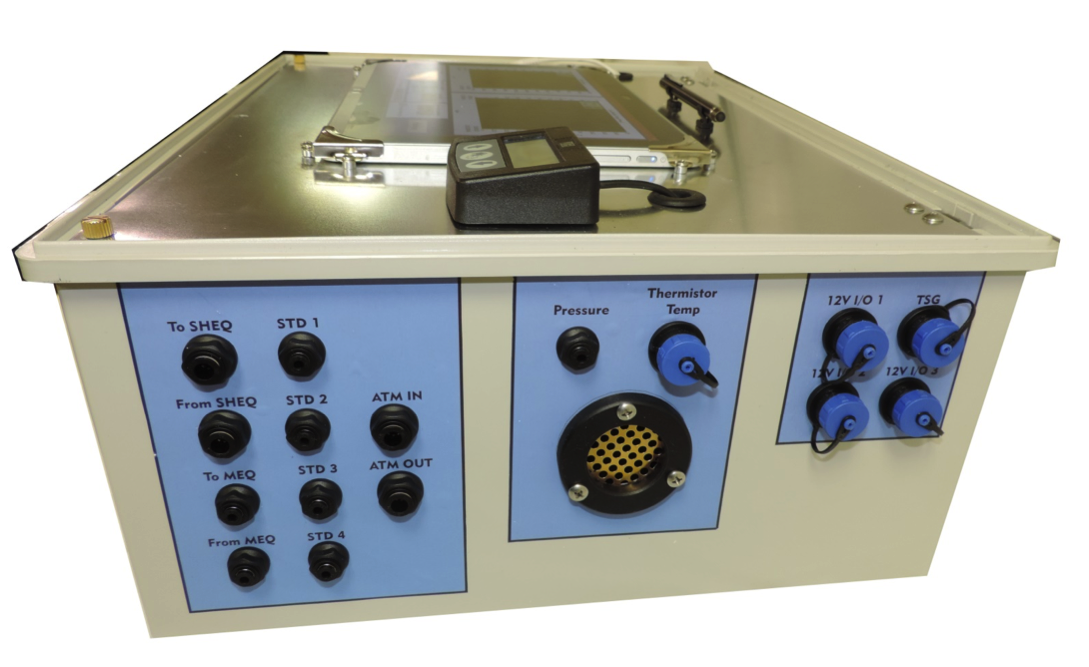
\includegraphics[width=7in, left]{Fig3.png}
	}
	\caption{External connections on the right side of the \super system.}
	\label{fig:Fig3}
	\end{figure}
	
\subsection{Flow Meter and Exhaust Port}

On the front of the unit (Figure \ref{fig:Fig2}) is a 0--250\,mL/min flow meter for verifying gas flow rates for the system, including atmospheric samples and standards.  Sample flow is set to $\sim$\,50\,mL/min, atmospheric and standard tank settings are set to $\sim$\,100\,mL/min. Flow rates greater than $\pm$\,10\,mL/min require internal adjustment of the corresponding flow control valve (see Figure \ref{fig:Fig4} ``Restriction Valves'').

The exhaust port is located near the flow meter.  Exhaust is located on the outside of the unit to prevent water that is accidentally drawn into the system from affecting internal components.  The user should not connect tubing or impede/restrict the flow out of the exhaust port as this can cause errors in the Licor\,840A readings and give false readings of flow rates.

	\begin{figure}[t]
	\centering
	\captionsetup{justification=justified,singlelinecheck=false}
	\hbox{	
		\hspace{-58mm}
		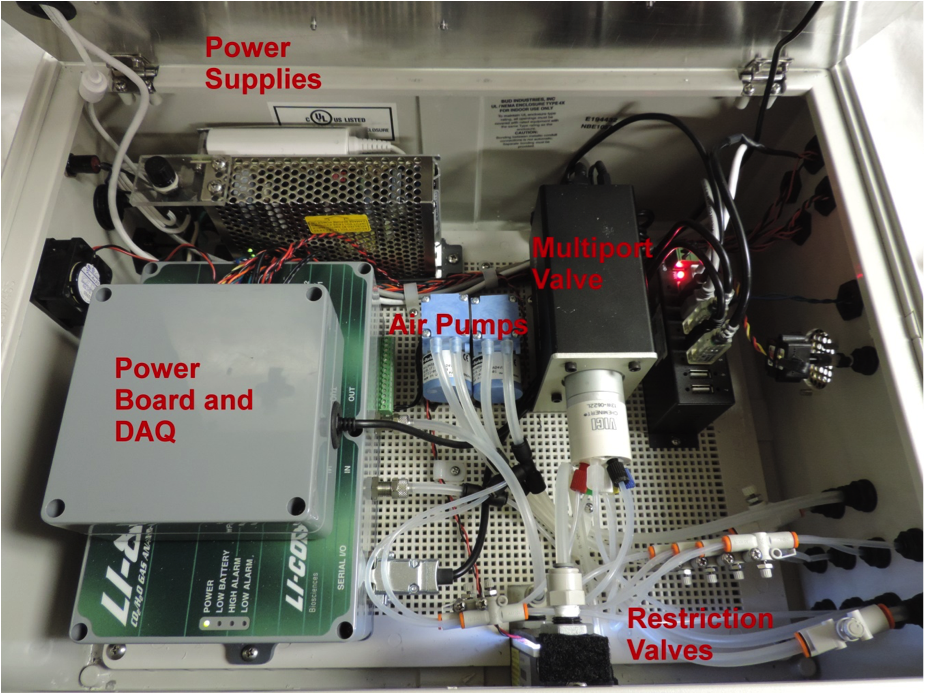
\includegraphics[width=7in, left]{Fig4.png}
	}
	\caption{View of internal components of the \super system.}
	\label{fig:Fig4}
	\end{figure}
	
\subsection{External Connections}

Figure \ref{fig:Fig3} shows the external connections on the right hand side of the \super system.  The system can be configured for either the showerhead or membrane equilibrator and requires minor changes in plumbing for each configuration.  (Please see Instrument Setup section below for details.)  The four standard connections connect to the user�s standard tanks.  The atmospheric IN connection connects, via tubing, to an external source of fresh atmospheric air.  In choosing a location for this in-take avoid vents from HVAC systems and similar sources of non-representative air.
	
The pressure sensor connects to a port in the top of the SHEQ or to the tee in the sample outlet of the MEQ.  The thermistor plugs into the 2-pin connection.  The three optional 12V\,I/O connections and Seabird SBE\,45 MicroTSG thermosalinograph connection are shown on the right. 


\subsection{Internal Components}

Figure \ref{fig:Fig4} shows a labeled view of the major interior components of the \super, including the power supplies, multi-port valve, Licor\,840A analyzer, two air pumps, pressure sensor, restriction valves, DAQ and power board enclosure.


\section{Instrument Setup}


\subsection{General Plumbing Overview}

Figure \ref{fig:Fig7} shows schematically how the system is plumbed for the showerhead equilibrator, while Figure \ref{fig:Fig9} shows the configuration for the contactor equilibrator.  In both arrangements, all gases flow through the multi-port valve (sample, atmospheric and standards) as shown in Figure \ref{fig:Fig6}.  Gas flows in through the selected port, out of the common center port and is plumbed to the input of the Licor\,840A.  All non-selected ports are closed off.


\vspace{3mm}
	\hbox{
		\hspace{-46mm}
		\begin{minipage}[h]{0.75\hsize}
			\floatbox[{\capbeside\thisfloatsetup{capbesideposition={left,top},capbesidewidth=4cm}}]{figure}[\FBwidth]
			{\caption{Connections to the VICI Multiport valve.}\label{fig:Fig5}}
			{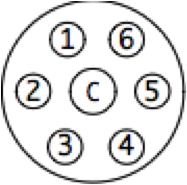
\includegraphics[scale=1.2, left]{Fig5.png}}
		\end{minipage}
		\noindent
			\begin{minipage}[h]{0.5\hsize}
			\begin{tabular}{c l}
				\toprule
				Port	&	Description\\
				\midrule
				1		&	From SHEQ/MEQ\\
				2		&	From ATM\\
				3		&	Standard 1\\
				4		&	Standard 2\\
				5		&	Standard 3\\
				6		&	Standard 4\\
				C		&	Output to Licor\,840A\\
				\bottomrule
			\end{tabular}
		\end{minipage}
	}
	

\subsection{Atmospheric Sample Plumbing}

The air-pumps run continuously ensuring the tubing is continuously flushed. Tubing for atmospheric air should be run so as to sample uncontaminated marine air.  On shipboard installations this would typically be run to the bow, avoiding exhaust gas and other non-representative air sources.

The air-pump outlet is equipped with a tee and restrictor (Figure \ref{fig:Fig4}) to direct $\sim$\,100\,mL/min to port 2 of the multiport valve.  Once the supply and exhaust tubing are in place the restrictor may require adjustment. This restriction valve has a locking nut that should be loosened before adjustment and then retightened.


\subsection{Standard Gas Plumbing}

The gas standards should be in regulated bottles set to approximately 25\,psig\,($\pm$\,10).  The pressure regulator or the restriction valves on each line can be adjusted if the gas flow is not correct (100\,mL/min\,$\pm$\,10).  These restriction valves have a locking nut to be loosened before adjustment and then retightened.


\subsection{Gas Drying}

If the sample gas dew point is above ambient temperature, you will need to dry the sample gas.  This can be accomplished with a peltier condenser, a Perma Pure PD-series nafion dryer with a heated inlet, or a large desiccant chamber such as the DRIERITE Laboratory Gas Drying Unit.  Contact Sunburst Sensors for technical support in implementing these options.

	
\subsection{Configuration for Showerhead Equilibrator}

The air-pump circulates $\sim$\,1000\,mL/min of air through the showerhead chamber equilibrating with the seawater in the sample stream $\sim$\,1\,gal/min.  A tee and restrictor in the return line diverts $\sim$\,50\,mL/min of this air to the Licor\,840A via port 1 of the multi-port valve.   This loss of loop air is made-up by drawing air back into the equilibrator.

	\begin{figure}[h]
	\hbox{
		\hspace{-54mm}
		\floatbox[{\capbeside\thisfloatsetup{capbesideposition={left,top},capbesidewidth=4cm}}]{figure}[\FBwidth]
		{\caption{SHEQ lid and SHEQ assembly.}\label{fig:Fig6}}
		{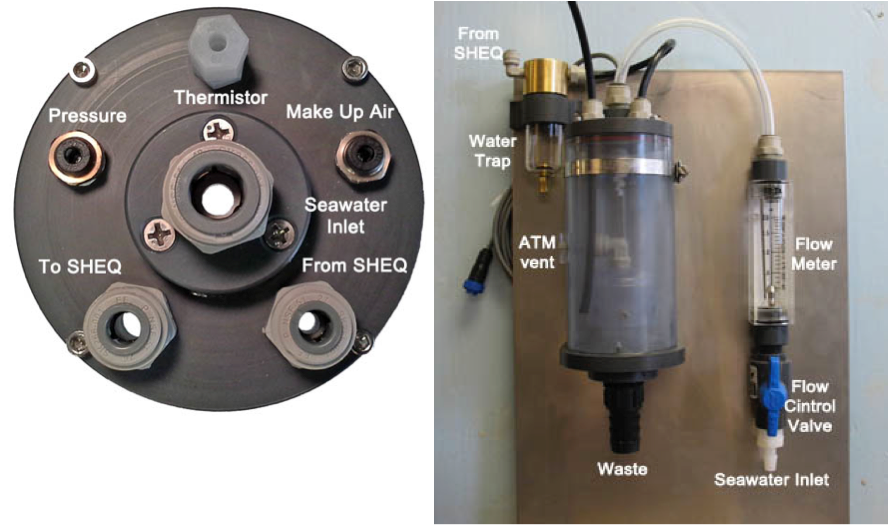
\includegraphics[width=\textwidth, left]{Fig6.png}}
	}
	\end{figure}

It is strongly suggested that the user use a tee from the atmospheric exhaust connection to supply this make-up air since air from around the system may be substantially higher in \dioxide due to human respiration or other sources.  Atmospheric air should be much closer to the sample�s p\dioxide.

\marginpar{\textcolor{red}{\textbf{\textsf{To prevent flooding, the seawater waste stream should drain to atmosphere with no interference.  Always connect the \textit{To SHEQ} line before connecting the \textit{From SHEQ} line as net negative pressure in the SHEQ can flood the system.}}}}

Remove the tubing connecting the \textit{From MEQ} enclosure port on the inside of the \super to position 1 of the multiport valve. Complete the conversion by removing the tubing that connects the restrictor valve and \textit{To MEQ} enclosure port on the inside of the \super and connect this restrictor valve to the port 1 of the multiport valve with the appropriately labeled tubing in the SHEQ conversion kit.

	\begin{figure}[h]
	\hbox{
		\hspace{-54mm}
		\floatbox[{\capbeside\thisfloatsetup{capbesideposition={left,top},capbesidewidth=4cm}}]{figure}[\FBwidth]
		{\caption{SHEQ plumbing.}\label{fig:Fig7}}
		{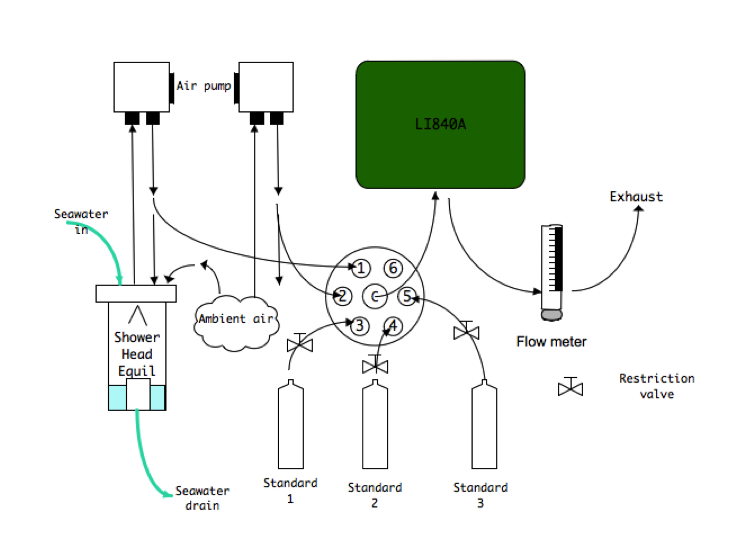
\includegraphics[width=\textwidth, left]{Fig7.png}}
	}
	\end{figure}

Connect tubing between \textit{To SHEQ} enclosure port to the tube in the lid of the equilibrator.   Complete the recirculation loop by connecting \textit{From SHEQ} enclosure port to the sample port in the water trap. Connect make-up air loop as described above. Connect pressure sensor tubing and finish by connecting the thermistor and seawater inlet.
	
	\begin{figure}[ht]
	\hbox{
		\hspace{-54mm}
		\floatbox[{\capbeside\thisfloatsetup{capbesideposition={left,top},capbesidewidth=4cm}}]{figure}[\FBwidth]
		{\caption{MEQ assembly.}\label{fig:Fig8}}
		{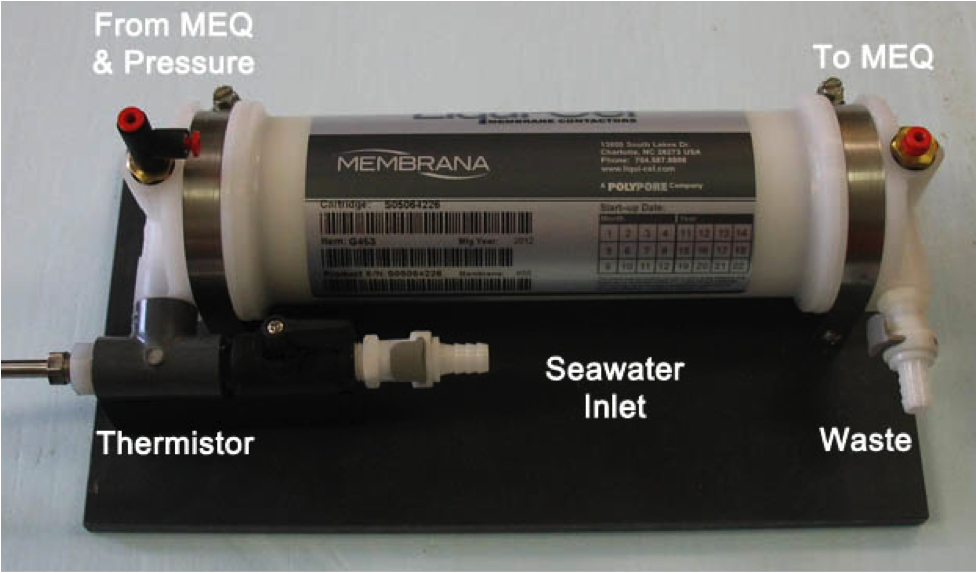
\includegraphics[width=\textwidth, left]{Fig8.png}}
	}
	\end{figure}

	
\subsection{Configuration for Membrane Equilibrator}

To use the MEQ configure the plumbing to match Figure \ref{fig:Fig8}.  In this arrangement there is no circulating loop and equilibration is accomplished in a single pass. The liquid stream and the gas stream are run anti-parallel increasing residence time in the MEQ.  Ambient air is drawn into the pump through the \textit{From SHEQ} enclosure port (Figure \ref{fig:Fig3}). The pump exhaust is equipped with a tee and restrictor valve.%
%
\marginpar{\textbf{\textsf{NOTE:  In restricting the liquid flow through the contactor, any restriction should be on the inlet side, as shown, to avoid pressurizing the contactor.}}}%
%
Remove the tubing that connects the restrictor valve and port 1 of the multiport valve and connect this restrictor valve to the \textit{To MEQ} enclosure port on the inside of the \super enclosure with the appropriately labeled tubing in the MEQ conversion kit.  Complete the conversion by connecting the \textit{From MEQ} enclosure port on the inside of the \super to position 1 of the multiport valve with the appropriately labeled tubing in the MEQ conversion kit.

To use the MEQ, connect the \textit{From MEQ} port on the right hand side of the \super enclosure to the tee on the contactor. Connect the \textit{To MEQ} port on the right hand side of the \super enclosure to the gas inlet on the contactor. Connect the Pressure enclosure port to the remaining port in the tee on the contactor.  Connect the thermistor lead to the \super.  Connect the seawater inlet to the MEQ and drain to atmosphere with no interference.

	\begin{figure}[h]
	\hbox{
		\hspace{-54mm}
		\floatbox[{\capbeside\thisfloatsetup{capbesideposition={left,top},capbesidewidth=4cm}}]{figure}[\FBwidth]
		{\caption{MEQ plumbing.}\label{fig:Fig9}}
		{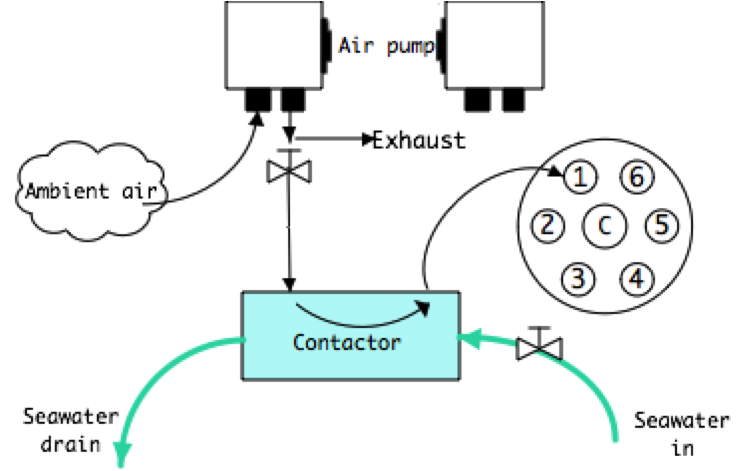
\includegraphics[width=\textwidth, left]{Fig9.png}}
	}
	\end{figure}

	
\subsection{Electrical Connections}

The \super supports a connection for a Seabird Thermosalinograph (SBE\,45) as well as up to three external instruments with analog output signals.  The pin-out of these connections and internal wire color is shown in Figure \ref{fig:Fig10}.  Note that for the TSG, the RX and TX of the \super should be connected to the TX and RX of the SBE\,45.  Also note that the SBE\,45 has a single ground used for both power and serial connection.

The electrical connections use the Bulgin 400 series connectors.  Mating cable construction requires the following Bulgin parts:

\begin{adjustwidth}{1cm}{}
	\begin{description}[before={\renewcommand\makelabel[1]{##1 ---}}]
		\item[PX0410/4S] Socket Connection, 4-position, Female
		\item[PX0483] Collet, Cable Gland
		\item[SA3348/1] Solder socket contacts
	\end{description}
\end{adjustwidth}

These parts and data sheets are available from Digi-Key Electronics \break (www.digikey.com). 

	\begin{figure}[h]
	\hbox{
		\hspace{-54mm}
		\floatbox[{\capbeside\thisfloatsetup{capbesideposition={left,top},capbesidewidth=4cm}}]{figure}[\FBwidth]
		{\caption{Pinouts for SBE\,45 MicroTSG or 12V\,I/O connections.}\label{fig:Fig10}}
		{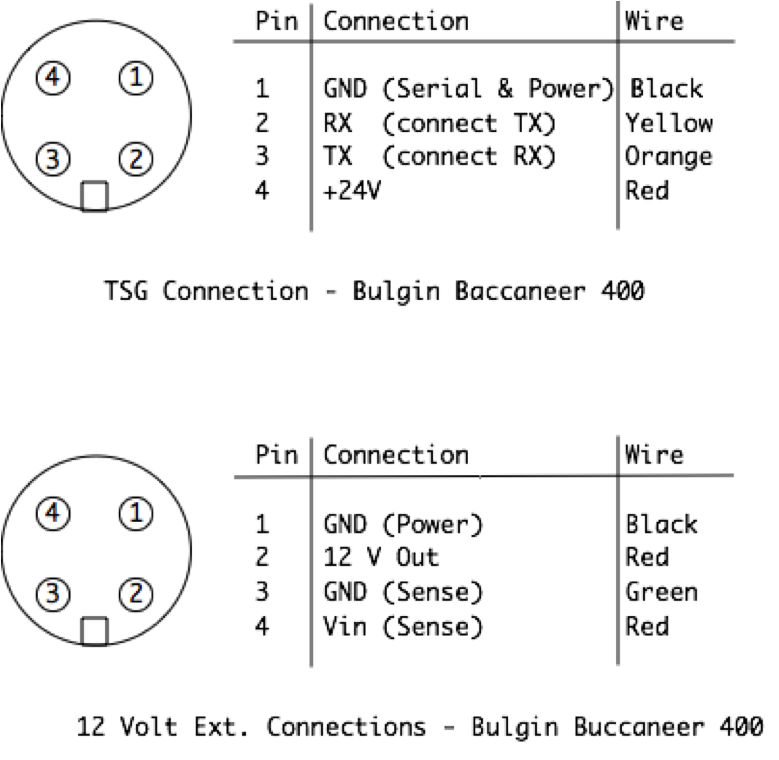
\includegraphics[width=\textwidth, left]{Fig10.png}}
	}
	\end{figure}
	
	\newpage


\subsection{Temperature and Pressure Sensors}

The temperature sensor precision is approximately 0.1 degree centigrade. %
\marginpar{\textsf{See enclosed \super Critical Information Sheet for sensor calibration information.}}%
%
The pressure sensor and temperature sensor have been calibrated in-house and the following equations are used to convert voltages where $V_{meas}$ is measured voltage, $T_C$ is measured temperature in degrees celcius, and $P_{abs}$ is measured pressure in kPa.

\subsubsection{Temperature sensor}

\begin{equation}
R_t = \frac{R1}{2.5/V_{meas} - 1}
\end{equation}

\begin{equation}
T^{-1} = A + B \ln R_t + C \ln {R_t}^3
\end{equation}

\begin{equation}
T_C = T^{-1} - 273.15
\end{equation}

\subsubsection{Pressure sensor}

\begin{equation}
P_{abs} = m V_{meas} + b
\end{equation}


\section{Software Setup and Operation}
	
	\begin{figure}[h!]
	\centering
	\captionsetup{justification=justified,singlelinecheck=false}
	\hbox{	
		\hspace{-58mm}
		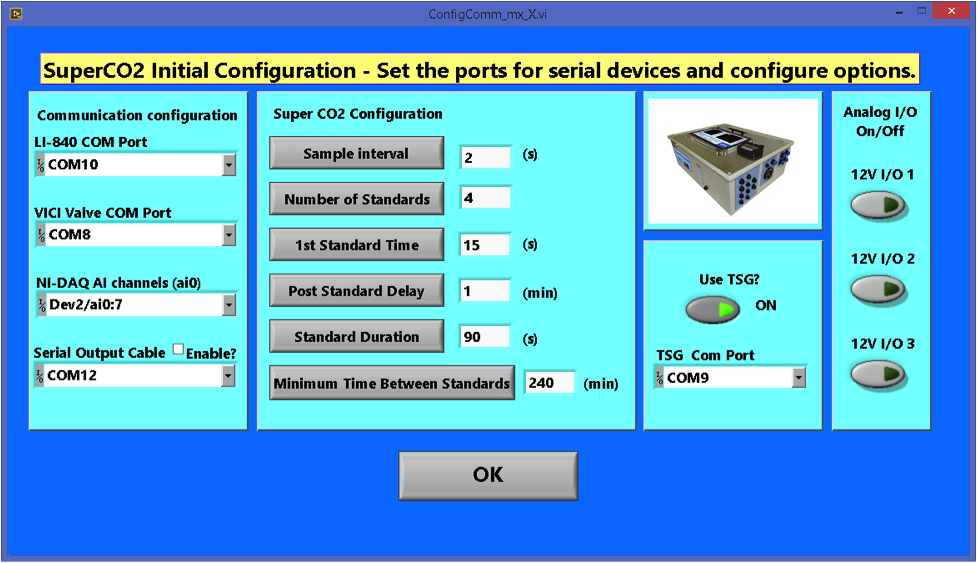
\includegraphics[width=7in, left]{Fig11.png}
	}
	\caption{Communication and instrument configuration panel.}
	\label{fig:Fig11}
	\end{figure}

\subsection{Communications Configuration}

Upon run of the \super application the \textit{ConfigComm} panel will appear and allow the user to set or confirm the communication settings and sampling interval.  (Figure \ref{fig:Fig11}) The \textit{LI-840 COM Port} control must point to the COM port for the Licor\,840A.  The \textit{VICI Valve COM Port} control must point to the COM port for the multiport valve.  The \textit{NI-DAQ AI channels} read similar to: ``DevX/ai0:7'' where ``X'' specifies the device number.

\marginlabel{\textit{Sample Interval}\,\,\,\,\,---}%
%
Sets the sampling interval for the system in seconds and determines how often data is written to file.  A minimum of two seconds is recommended.  This is the only place to adjust the sample interval.

\marginlabel{\textit{Number of Standards}\,\,\,\,\,---}%
%
Tells the \super how many standards are connected.  It is assumed they will be connected starting with position 2 and ascending. This value can be changed in real time.

\marginlabel{\textit{1st Standard Time}\,\,\,\,\,---}%
%
Sets the time, in minutes, after which the first standard will run.  This allows time for setup and Licor\,840A temperature stabilization.  This value can be changed in real time.

\marginlabel{\textit{Standard Duration}\,\,\,\,\,---}%
%
Sets the length of time, in seconds, that each standard will be turned on and monitored.  This should be set long enough that the standard readings stabilize, but not so long as to waste gas.  Settings between 60 and 300 seconds are typical.  This value can be changed in real time. 

\marginlabel{\textit{Post Standard Delay}\,\,\,\,\,---}%
%
Sets the delay, in minutes, after the standards and atmospheric sample have been run.  This gives the equilibrator system time to stabilize before recording resumes. This value can be changed in real time.

\marginlabel{\textit{Minimum Time Between Standards}\,\,\,\,\,---}%
%
Sets the number of minutes between standards sequences.  Typically standards should be run every four to six hours. This value can be changed in real time.

\marginlabel{\textit{Use TSG?}\,\,\,\,\,---}%
%
If a Seabird thermosalinograph is attached to the system, turn on the switch here and specify the COM port assigned to the device.

\marginlabel{\textit{Analog I/O}\,\,\,\,\,---}%
%
If any 12\,V external instruments are connected to the system, turn on the appropriate switch here to log their voltages.

Once these settings have been set correctly, click the \textit{OK} button.  The software writes these settings to a preference file so no change is required thereafter unless there has been a change to the system (e.g. the addition of a TSG).


\subsection{Output File Directory}

The next dialog box to appear allows the user to create and select the output file directory and the raw data root file name. Clicking \textit{OK} will initialize the program to the preferences written with the \textit{ConfigComm} dialog.

	\begin{figure}[h]
	\hbox{
		\hspace{-54mm}
		\floatbox[{\capbeside\thisfloatsetup{capbesideposition={left,top},capbesidewidth=4cm}}]{figure}[\FBwidth]
		{\caption{Output directory dialog.}\label{fig:Fig12}}
		{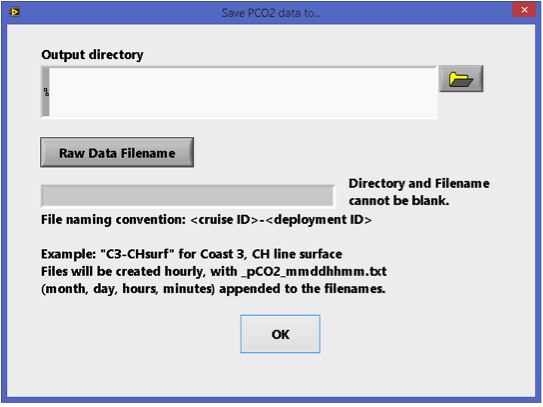
\includegraphics[width=\textwidth, left]{Fig12.png}}
	}
	\end{figure}

%\newpage

\section{System User Interface}

When launched, the program will operate under the default settings in the user interface shown in Figure \ref{fig:Fig11}. The settings and information clusters are discussed below. When running, some of these settings can be changed in real time.

	\begin{figure}[h!]
	\centering
	\captionsetup{justification=justified,singlelinecheck=false}
	\hbox{	
		\hspace{-58mm}
		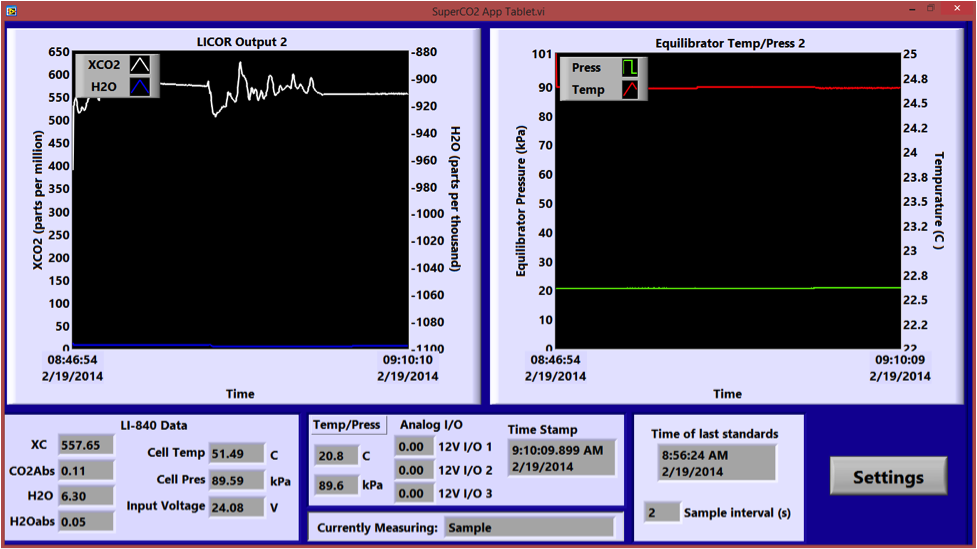
\includegraphics[width=7in, left]{Fig13.png}
	}
	\caption{The system user interface showing the Data Display window at startup.}
	\label{fig:Fig13}
	\end{figure}

\subsection{Data Display Window}


\subsubsection{LICOR Output Panel}

The \textit{LICOR Output} panel displays the X\dioxide in parts per million and \water content in parts per thousand of the sample gas stream as a function of time.

	\begin{figure}[h]
	\hbox{
		\hspace{-25mm}
		\floatbox[{\capbeside\thisfloatsetup{capbesideposition={right,top},capbesidewidth=6cm}}]{figure}[\FBwidth]
		{\captionsetup{labelformat=empty}
		\caption{The Licor\,840A outputs data in XML format via RS-232.  The \super client software parses the data and presents it in this cluster as well as plotting measured X\dioxide and \water parameters.  A brief description of each quantity is given in Table \ref{DataTab} below.  For in-depth discussion of the Licor\,840A function, please consult its manual.}\label{fig:Fig14}}
		{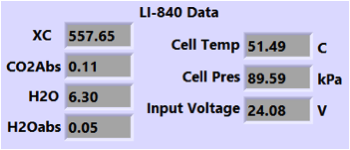
\includegraphics[width=0.6\textwidth, right]{Fig14.png}}
	}
	\end{figure}


\subsubsection{Equilibrator Temperature and Pressure Panel}

This \textit{Equilibrator} panel displays the seawater temperature in the SHEQ/MEQ in degrees celcius as well as the equilibrator pressure in kPa as a function of time. For both charts, the y-axis is auto scaled.  The time domain is determined by the \textit{Display Scale} (min) control cluster described below.

	\begin{figure}[h]
	\hbox{
		\hspace{-25mm}
		\floatbox[{\capbeside\thisfloatsetup{capbesideposition={right,top},capbesidewidth=6cm}}]{figure}[\FBwidth]
		{\captionsetup{labelformat=empty}
		\caption{The \textit{Analog\,I/O} cluster is for reading equilibrator temperature (C) and pressure (kPa) in the equilibrator.  The time stamp updates with each reading. If external 12\,V instruments were selected in the \textit{ConfigComm} dialog, their voltages will display here.}\label{fig:Fig15}}
		{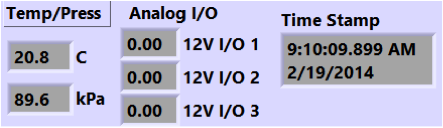
\includegraphics[width=0.6\textwidth, right]{Fig15.png}}
	}
	\end{figure}

\FloatBarrier


\subsection{Settings Window}

	\begin{figure}[h]
	\hbox{
		\hspace{-25mm}
		\floatbox[{\capbeside\thisfloatsetup{capbesideposition={right,top},capbesidewidth=6cm}}]{figure}[\FBwidth]
		{\captionsetup{labelformat=empty}
		\caption{Displays the time stamp of the last standards and the sample interval. Pressing the \textit{Settings} button switches the view to the \textit{Settings} window (see Figure \ref{fig:Fig17}).}\label{fig:Fig16}}
		{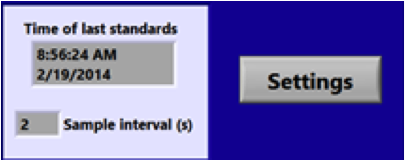
\includegraphics[width=0.6\textwidth, right]{Fig16.png}}
	}
	\end{figure}

	\begin{figure}[htbp!]
	\centering
	\captionsetup{justification=justified,singlelinecheck=false}
	\hbox{	
		\hspace{-58mm}
		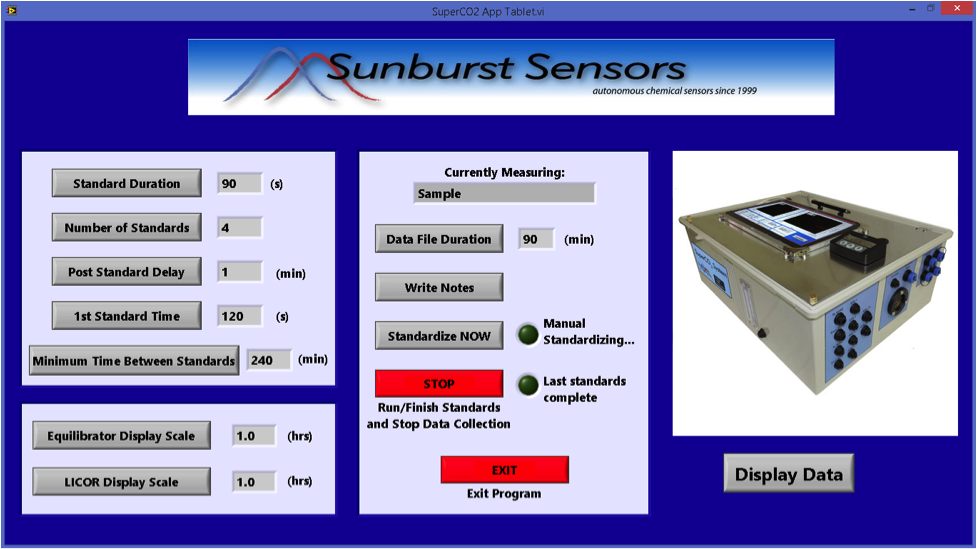
\includegraphics[width=7in, left]{Fig17.png}
	}
	\caption{The system user interface showing the Settings window.}
	\label{fig:Fig17}
	\end{figure}

	\begin{figure}[h!]
	\hbox{
		\hspace{-25mm}
		\floatbox[{\capbeside\thisfloatsetup{capbesideposition={right,top},capbesidewidth=6cm}}]{figure}[\FBwidth]
		{\captionsetup{labelformat=empty}
		\caption{Sets the x-axis length of time prior to current measurement of the \textit{LICOR Output} and \textit{Equilibrator} panels. These values can be changed in real time.}\label{fig:Fig18}}
		{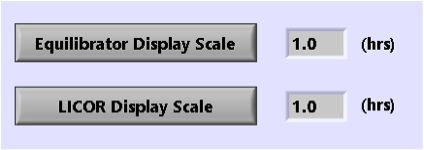
\includegraphics[width=0.6\textwidth, right]{Fig18.png}}
	}
	\end{figure}

	\begin{figure}[h!]
	\hbox{
		\hspace{-25mm}
		\floatbox[{\capbeside\thisfloatsetup{capbesideposition={right,top},capbesidewidth=6cm}}]{figure}[\FBwidth]
		{\captionsetup{labelformat=empty}
		\caption{The controls in this cluster set parameters for gas standards used by the \super system.}\label{fig:Fig19}}
		{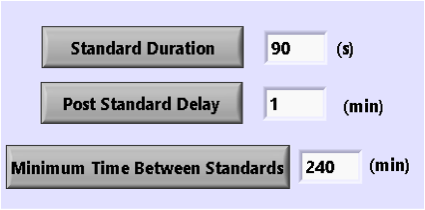
\includegraphics[width=0.6\textwidth, right]{Fig19.png}}
	}
	\end{figure}


\subsubsection{Settings Window Parameters}
	
\marginlabel{\textit{Standard Duration}\,\,\,\,\,---}%
%
Sets the length of time, in seconds, that each standard will be turned on and monitored.  This should be set long enough that the standard readings stabilize, but not so long as to waste the gas.  Settings between 60 and 300 seconds are typical.  This value can be changed in real time.

\marginlabel{\textit{Post Standard Delay}\,\,\,\,\,---}%
%
Sets the delay in minutes after the standards and atmospheric sample have been run.  This gives the equilibrator system time to stabilize before recording resumes. This value can be changed in real time.

\marginlabel{\textit{Minimum Time Between Standards}\,\,\,\,\,---}%
%
Sets the number of minutes between standards sequences.  Typically standards should be run every four to six hours. This value can be changed in real time.

	\begin{figure}[h]
	\hbox{
		\hspace{-25mm}
		\floatbox[{\capbeside\thisfloatsetup{capbesideposition={right,top},capbesidewidth=6cm}}]{figure}[\FBwidth]
		{\captionsetup{labelformat=empty}
		\caption{The controls in this cluster are for setting the file length and stop control of the instrument.}\label{fig:Fig20}}
		{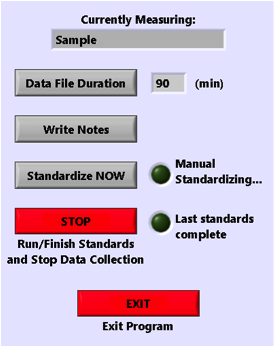
\includegraphics[width=0.6\textwidth, right]{Fig20.png}}
	}
	\end{figure}

\marginlabel{\textit{Currently Measuring}\,\,\,\,\,---}%
%
Displays the current position of the multiport valve.

\marginlabel{\textit{Data File Duration}\,\,\,\,\,---}%
%
Sets the file length in minutes and can be changed in real time.

\marginlabel{\textit{Write Notes}\,\,\,\,\,---}%
%
Allows time stamped notes to be recorded and saved in separate file.

\marginlabel{\textit{Standardize NOW}\,\,\,\,\,---}%
%
Runs the standard sequence manually upon button press.

\marginlabel{\textit{STOP}\,\,\,\,\,---}%
%
When pressed will run or finish a gas standards sequence and stops data collection.

\marginlabel{\textit{Manual Standardizing...}\,\,\,\,\,---}%
%
Indicates a manual standard sequence is currently running.

\marginlabel{\textit{Last Standards Complete}\,\,\,\,\,---}%
%
Indicates when the last standards sequence has been completed.

\marginlabel{\textit{EXIT}\,\,\,\,\,---}%
%
When pressed will shut down the program immediately.



\subsection{Output File Structure}

Data generated from the \super system is saved in a tab delineated text file (*.txt).  There are five header lines including the column titles.  Data and corresponding labels are tab-delimited in the file.  Figure \ref{fig:Fig12} is an example data file; this example demonstrates the valve changing position from seawater to atmospheric, standards 1 through 3, and back to seawater. For TSG columns, ``NaN'' indicates the equipment is not currently attached to the system.  The analog inputs IO3, IO4 and IO5 display ``0'' if not in use.

	\begin{table}[h]
	\begin{center}
	\caption{\label{DataTab}Data file header descriptions.}
	\vspace{3mm}
	\centering
	\begin{tabular}{r l}
		\toprule
		Column Title	&	Description\\
		\midrule
		DOY{\_}UTC	&	System time (UTC\,+\,0)\\
		CO2{\_}ppm	&	Mole fraction of \dioxide  in parts per million\\
		CO2{\_}abs	&	\dioxide absorption\\
		H20{\_}ppt	&	Mole fraction of \water in parts per thousand\\
		H20{\_}abs	&	\water absorption\\
		Cell{\_}T		&	Optical cell temperature\\
		Cell{\_}P		&	Optical cell pressure\\
		820pwrV		&	Input voltage reading in volts\\
		Temp (C)		&	Temperature sensor reading in {$^\circ$}\,C\\
		Press (kPa)	&	Pressure sensor reading in kPa\\
		Temp (V)		&	Temperature sensor reading in volts\\
		Press (V)		&	Pressure sensor reading in volts\\
		IO3			&	Analog input 1 in volts\\
		IO4			&	Analog input 2 in volts\\
		IO5			&	Analog input 3 in volts\\
		valve1pos		&	Valve position\\
		TSG{\_}T		&	TSG temperature output\\
		TSG{\_}S		&	TSG salinity output\\
		Date			&	Date of data aquisition\\
		Time			&	Time of data aquisition\\
		\bottomrule
	\end{tabular}
	\end{center}
	\end{table}

	\begin{figure}[h!]
	\centering
	\captionsetup{justification=justified,singlelinecheck=false}
	\hbox{	
		\hspace{-58mm}
		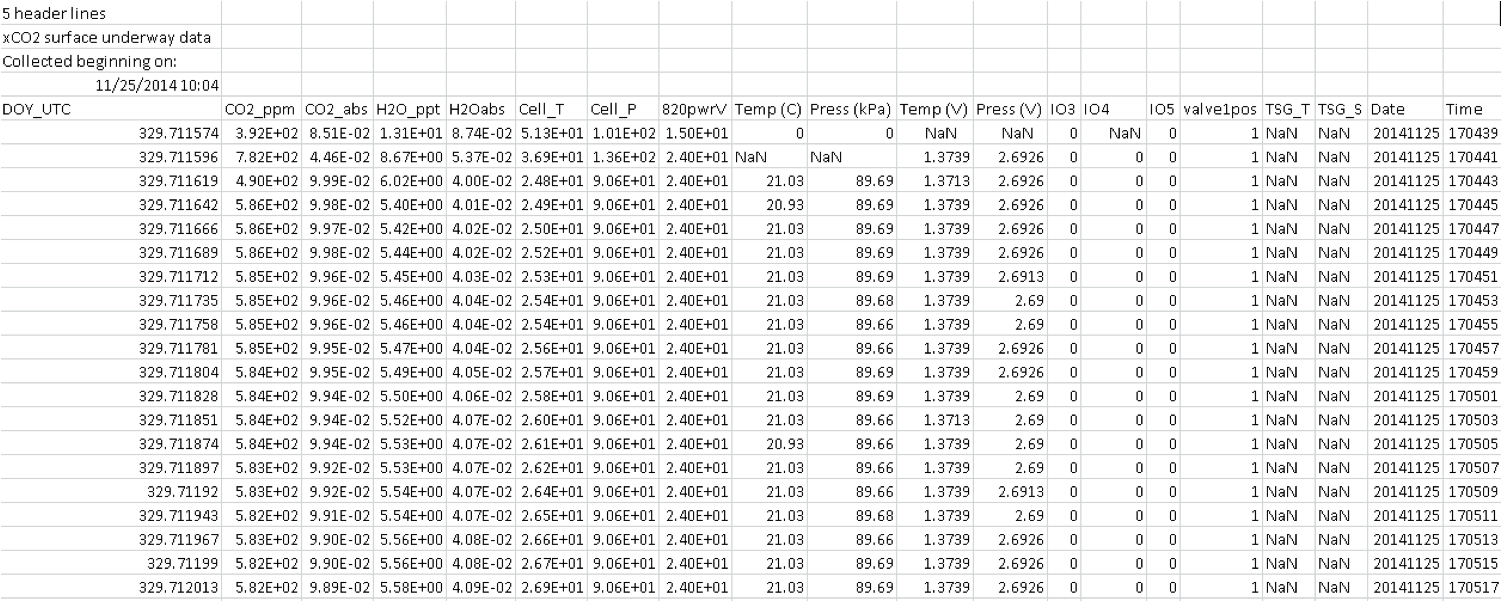
\includegraphics[width=7in, left]{Fig21.png}
	}
	\caption{Example output file.}
	\label{fig:Fig21}
	\end{figure}

\newpage


\begin{fullpage}

\section{Warranty}

\footnotesize

SUNBURST WARRANTS HARDWARE PRODUCTS TO BE FREE FROM DEFECTS IN MATERIAL AND WORKMANSHIP FOR 1 YEAR FROM DATE OF SHIPMENT. LIABILITY UNDER THIS WARRANTY IS LIMITED TO REPAIR OR REPLACEMENT OF DEFECTIVE PARTS AND PRODUCTS, WHICH MUST BE RETURNED WITH AN RMA NUMBER OBTAINED FROM SUNBURST PRIOR TO SHIPMENT.  SHIPPING COSTS AND RISK OF LOSS SHALL BE BORNE BY CUSTOMER.  SUNBURST HAS THE OPTION OF REPAIRING OR REPLACING THE RETURNED ITEM(S).  AFTER 1 YEAR, REPAIR AND REPLACEMENT IS OFFERED ONLY UPON PAYMENT BY CUSTOMER OF FULL PRICE OF PARTS AND LABOR FOR SAID REPAIRS.

SUNBURST OWNS ALL PARTS REMOVED FROM REPAIRED PRODUCTS. SUNBURST MAY USE NEW AND/OR RECONDITIONED PARTS IN PERFORMING WARRANTY REPAIRS AND BUILDING REPLACEMENT PRODUCTS. PRICES OF THE PART REPLACED WILL BE AT SUNBURST'S THEN CURRENT STANDARD PRICE.
 
SUNBURST DOES NOT WARRANT THAT THE PRODUCTS ARE FIT FOR ANY PARTICULAR PURPOSE AND THE WARRANTY HEREIN IS GIVEN IN PLACE OF ALL WARRANTIES, CONDITIONS, TERMS, UNDERTAKINGS AND OBLIGATIONS IMPLIED BY STATUTE, COMMON LAW, TRADE USAGE, COURSE OF DEALING OR OTHERWISE INCLUDING WARRANTIES OR CONDITIONS OF MERCHANTABILITY, FITNESS FOR PURPOSE, SATISFACTORY QUALITY AND/OR COMPLIANCE WITH DESCRIPTION, ALL OF WHICH ARE HEREBY EXCLUDED TO THE FULLEST EXTENT PERMITTED BY LAW.
 
THE CUSTOMER AGREES THAT, IN RELATION TO THIRD PARTY PRODUCTS PURCHASED THROUGH SUNBURST, WHERE SUCH OF THE PRODUCTS ARE COVERED BY A RELEVANT MANUFACTURER'S WARRANTY, THEN THE WARRANTY SHALL NOT EXTEND TO SUCH PRODUCTS AND SUCH MANUFACTURER'S WARRANTY SHALL BE THE SOLE WARRANTY IN RESPECT OF SUCH PRODUCTS. THE CUSTOMER SHALL UTILIZE THAT WARRANTY FOR THE SUPPORT OF SUCH PRODUCTS AND IN ANY EVENT NOT LOOK TO SUNBURST FOR SUCH WARRANTY SUPPORT. 

THIS WARRANTY (AND ANY QUALIFICATION TEST REPORTS SUBMITTED BY SUNBURST TO CUSTOMER) IS NOT, AND SHALL NOT BE CONSTRUED AS A GUARANTEE OF PEAK PERFORMANCE OF THE PRODUCTS SUPPLIED HEREUNDER FOR THE ENTIRE WARRANTY PERIOD.

SUNBURST DOES NOT WARRANT ACCESSORIES AND PERIPHERAL DEVICES THEREOF FURNISHED BY CUSTOMER OR OBTAINED FROM OTHER MANUFACTURERS OR SUPPLIED AT CUSTOMER�S REQUEST AND/OR TO CUSTOMER�S SPECIFICATION, EXCEPT TO THE EXTENT THAT THE ORIGINAL MANUFACTURER OR SUPPLIER THEREOF EXPRESSLY GUARANTEES OR WARRANTS SUCH PRODUCTS OR PARTS THEREOF. SUNBURST ASSUMES NO RESPONSIBILITY OR LIABILITY FOR THE ADEQUACY OF ANY DESIGN, SPECIFICATION, DRAWING OR MATERIAL FURNISHED OR SPECIFIED BY CUSTOMER.

THIS WARRANTY DOES NOT COVER DAMAGE, FAULT, FAILURE OR MALFUNCTION DUE TO EXTERNAL CAUSES, INCLUDING ACCIDENT, ABUSE, MISUSE, NEGLECT, PROBLEMS WITH ELECTRICAL POWER, SERVICING NOT AUTHORIZED BY SUNBURST, USAGE AND/OR STORAGE AND/OR INSTALLATION NOT IN ACCORDANCE WITH PRODUCT INSTRUCTIONS, FAILURE TO PERFORM REQUIRED PREVENTIVE MAINTENANCE, NORMAL WEAR AND TEAR, ACT OF GOD, FIRE, FLOOD, WAR, ACT OF VIOLENCE OR ANY SIMILAR OCCURRENCE; ANY ATTEMPT BY ANY PERSON OTHER THAN SUNBURST PERSONNEL OR ANY PERSON AUTHORIZED BY SUNBURST, TO ADJUST, REPAIR OR SUPPORT THE PRODUCTS AND PROBLEMS CAUSED BY USE OF PARTS AND COMPONENTS NOT SUPPLIED BY SUNBURST. THIS WARRANTY DOES NOT COVER ANY ITEMS THAT ARE IN ONE OR MORE OF THE FOLLOWING CATEGORIES: SERVICES; SOFTWARE; EXTERNAL DEVICES, ACCESSORIES OR PARTS ADDED TO THE PRODUCT AFTER THE PRODUCT IS SHIPPED FROM SUNBURST.

`CONSUMABLE' PARTS ARE NOT COVERED BY THIS WARRANTY AFTER THE UNIT HAS BEEN DEPLOYED OR USED.  THE FOLLOWING PARTS ARE CONSIDERED `CONSUMABLES' AND WILL BE REPLACED AT CUSTOMERS COST (INCLUDING LABOR) IF AND WHEN THE UNIT IS REFURBISHED BY SUNBURST:  N/A

REPLACEMENT OR REPAIR OF A PRODUCT OR COMPONENT THEREOF SUPPLIED HEREUNDER DOES NOT EXTEND THE ORIGINAL WARRANTY PERIOD OF THE PRODUCT OR COMPONENT BEING CORRECTED.

\end{fullpage}



\begin{comment}
%%%%%%%%%%%%%%%%%%%%%%%%%%%%%%%%%%%%%%
%%%%%%%%%%%%%%%%%%%%%%%%%%%%%%%%%%%%%%
%%%%%%%%%%%%%%%%%%%%%%%%%%%%%%%%%%%%%%

\begin{thebibliography}{}
\expandafter\ifx\csname natexlab\endcsname\relax\def\natexlab#1{#1}\fi
\expandafter\ifx\csname selectlanguage\endcsname\relax
  \def\selectlanguage#1{\relax}\fi

\bibitem[Wall, 2014]{Wall2014}
Wall, C.~M. (2014)
{Autonomous in situ measurements of estuarine surface P\dioxide: instrument development and initial estuarine observations.} (MS thesis, Oregon State University)

\bibitem[Moran, 2010]{Moran2010}
Moran, D. (2010)
{Carbon dioxide degassing in fresh and saline water. II: Degassing performance of an air-lift.} \textit{Aquacult. Eng.}, {\bf 43}(2010), 120--127.
  
\end{thebibliography}

%%%%%%%%%%%%%%%%%%%%%%%%%%%%%%%%%%%%%%
%%%%%%%%%%%%%%%%%%%%%%%%%%%%%%%%%%%%%%
%%%%%%%%%%%%%%%%%%%%%%%%%%%%%%%%%%%%%%
\end{comment}


\end{document}